\section{LGBM}
LGBM, Microsoft tarafından 2017 yılında geliştirilmiştir. Modelin tanıtıldığı "LightGBM: A Highly Efficient Gradient Boosting Decision Tree" makalesinde diğer modellere göre 20 kat daha hızlı çalıştığı yazmaktadır. Diğer makine öğrenmesi modellerinden farklı olarak paralel öğrenme ve GPU kullanımını destekler. Light Gradient Boosting Machine, histogram tabanlıdır.  Kategorik değişkenler içn histogramı sıralar ve en iyi bölünmeyi seçer. Gradient boosting yöntemini kullanır. Ağaçları düşey olarak büyütür. Bu, her ağacın yalnızca veri kümesinin belirli bir alt kümesinde odaklanmasını sağlar böylece hesaplama süresi azalır.  Genelde karar ağacı algoritmaları seviye odaklı (level-wise - BFS) büyüme stratejisi kullanırken LGBM yaprak odaklı (leaf-wise - DFS) büyüme stratejisi kullanır. Yaprak odaklı büyümede bölme işlemi kaybı azalan yapraklardan devam eder. Böylece model daha az hata oranı ile daha hızlı öğrenir.

\begin{figure}[h]
    \centering
    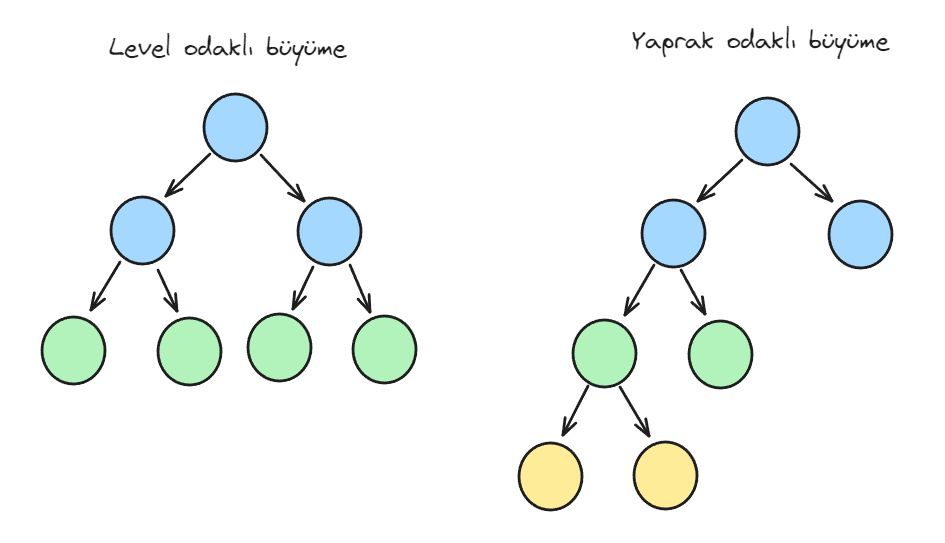
\includegraphics[width=1\textwidth]{images/grow_strategies.png}
    \caption{Büyüme stratejileri.}
    \label{fig:enter-label}
\end{figure}

Eğitim aşamasında 2 farklı yöntem barındırır.
\begin{itemize}
    \item \textbf{Gradient-based One-Side Sampling (GOSS):} Eğitim sürecinde kullanılan bir örnekleme tekniğidir. GOSS, büyük gradyanlara sahip örnekleri korurken, küçük gradyanlara sahip örnekleri filtreleyerek veri setinin boyutunu azaltır. Böylece gradient boost algoritması daha hızlı çalışır.
    \item \textbf{Exclusive Feature Bundling (EFB):} Özellik mühendisliği sırasında kullanılan bir tekniktir. EFB, benzer davranış gösteren özellikleri gruplayarak bellek kullanımını azaltır ve modelin karmaşıklığını azaltır. Yani seyrek özellikleri birleştirip daha yoğun özellikler oluşturur. Bu sayede, eğitim süresi kısaltılır ve modelin genelleştirme yeteneği artar.
\end{itemize}

\subsection{Hiperparametreler}
\begin{table}[h]
\centering
{\scriptsize\renewcommand{\arraystretch}{0.4}
{\resizebox*{\linewidth}{0.4\textwidth}{
\begin{tabular}{|p{3cm}|p{1cm}|p{1cm}|p{6cm}|}
\hline
Parametre & Type & Default & Açıklama \\ \hline
num\_leaves & int & 31 & Bir ağaçtaki her seviyedeki maksimum yaprak sayısı. Overfitting olmaması için $2^\text{max\_depth}$ den küçük olmalıdır.\\ \hline
max\_depth & int & -1 & Bir ağacın maksimum derinliği. \\ \hline
learning\_rate & int & 0.1 & Gradient güncellemeleri sırasında kullanılan öğrenme oranı. \\ \hline
n\_estimators & int & 100 & Oluşturulacak ağaç sayısı. \\ \hline
min\_child\_samples & int & 20 & Bir yaprağın altındaki minimum örnek sayısı. \\ \hline
subsample & int & 1 & Her ağaç için kullanılacak alt örnekleme oranı. \\ \hline
colsample\_bytree & int & 1 & Her ağaç için kullanılan özelliklerin yüzdesi. \\ \hline
reg\_alpha & int & 0 & L1 düzenleme. \\ \hline
reg\_lambda & int & 0 & L2 düzenleme. \\ \hline

\end{tabular}
}}}
\end{table}

\newpage